\chapter{Problem}
%Problem/Uppgift.
%Det här avsnittet är ofta den viktigaste delen av planeringsrapporten (och av den slutgiltiga uppsatsen/rapporten). Den syftar till att identifiera frågan/frågorna som ska tas upp i projektet. Det är viktigt att gruppen gör en problemanalys även om det i projektförslaget redan finns ett problem (en uppgift) specificerat. Anledningen till detta är att det riktiga primära problemet ofta skiljer sig från det i början av uppdragsgivaren/förslagsställaren/kunden föreslagna. Problemanalysen syftar också till att bryta ner problemet/uppgiften i mindre och mer detaljerade delproblem/deluppgifter, vilket också leder till formulering av delsyften. Genom att göra detta får studenterna mycket bättre förståelse för de olika aspekterna av problemet/uppgiften. Utan den här informationen är det omöjligt att identifiera vilken information som behövs, vilka informationskällor som behövs och lämpliga tillvägagångssätt.

%Avgränsningar
%Avgränsningarna ska ta upp vilka delar av problemet som inte tas upp i uppsatsen/rapporten, och anledningen till detta. Motivering av avgränsningarna är viktigt.

%Project description
%The task is to program an emulator application that can read the ROM extracted from an old console game cartridge, and emulate the hardware that would run the data contained in it, displaying the graphical output the hardware would have, and providing remapped input to the user to interact with the buttons that were in the hardware, allowing them to play the game. Focus will be to have a graphical interface working, not taking sound or other systems into account.

%\begin{itemize}
 %   \item Kan gruppen skapa en fungerande Game Boy-emulator? - relatera till projektbeskrivningen.
  %  \item Anpassa ny hårdvara att kunna köra gammal mjukvara?
   % \item MVP
%\end{itemize}


The original problem is to program an emulator which can read the ROM extracted from an old Game Boy game cartridge. Thereafter the emulator should be able to run the data contained within the cartridge and reproduce the experience of playing the original game. This includes displaying the graphical output and providing remapped input to the user to interact with the game. From this it is possible to derive multiple sub-problems in emulating and reproducing the behaviours of all hardware components. The greatest challenge with this problem is to emulate games built for a specific set of hardware, which are magnitudes slower than modern hardware, and yet make them run in speed truthful to the original hardware.
\\\\
The approach taken to the problem is to first research the hardware of the Game Boy, to be able to make a high-level design, and thereafter implement each component in a basic form. The design will roughly follow the hardware modules of the Game Boy which is further discussed below. Due to the fact that there is no official hardware documentation of the Game Boy publicly available, the the design of the emulator will have to rely on third party sources. Mainly the experiences of other developers and enthusiasts, such as Pan Docs\cite{pandocs}, Gekkio's Complete Technical Reference\cite{CompleteTechnicalReference} and the Wikipedia of Game Boy development; GBDev\cite{GBDev}.

%\todo{From original project description}
   % The task is to program an emulator application that can read the ROM extracted from an old Game Boy game cartridge, and emulate the hardware that would run the data contained in it, displaying the graphical output the hardware would have, and providing remapped input to the user to interact with the buttons that were in the hardware, allowing them to play the game. Focus will be to have a graphical interface working, not taking sound or other systems into account.

% https://gbdev.io/gb-opcodes/optables/ all opcodes.
% https://gbdev.io/pandocs/#memory-map
\section{Emulating the different parts of a Game Boy}
A Game Boy's hardware is split into different modules which each have a specific task. Each of these modules must therefore be emulated and assembled in code such that the Game Boy functionality matches the original. This can be done either by exactly replicating the specifications of the hardware in code, or by making simplifications with risk of losing some minor functionality. 
    
\subsection{Emulating the Central Processing Unit}
The Central Processing Unit (CPU) is one of the core modules which must be emulated. There are a set of 245 simple instructions\cite{Optable} which executes all calculations and logical operations as well as reading and writing to memory. Without the CPU, the Game Boy would not work at all and the implementation of the CPU is therefore one of the main problems to be solved.% It is also within the CPU the challenge of reproducing the working speed of the hardware will be handled, which, as previously mentioned is another central part.


\subsection{The Memory Unit}
The memory unit of the Game Boy consists of a single address space split into multiple sub-modules, each handling memory for different parts of the hardware, see figure \ref{fig:Memory-fig}. Instead of handling these as individual components, these can be emulated with a central Memory Management Unit, aka  MMU, which emulates the sub-modules in software.

  \begin{figure}[H]
    \centering
    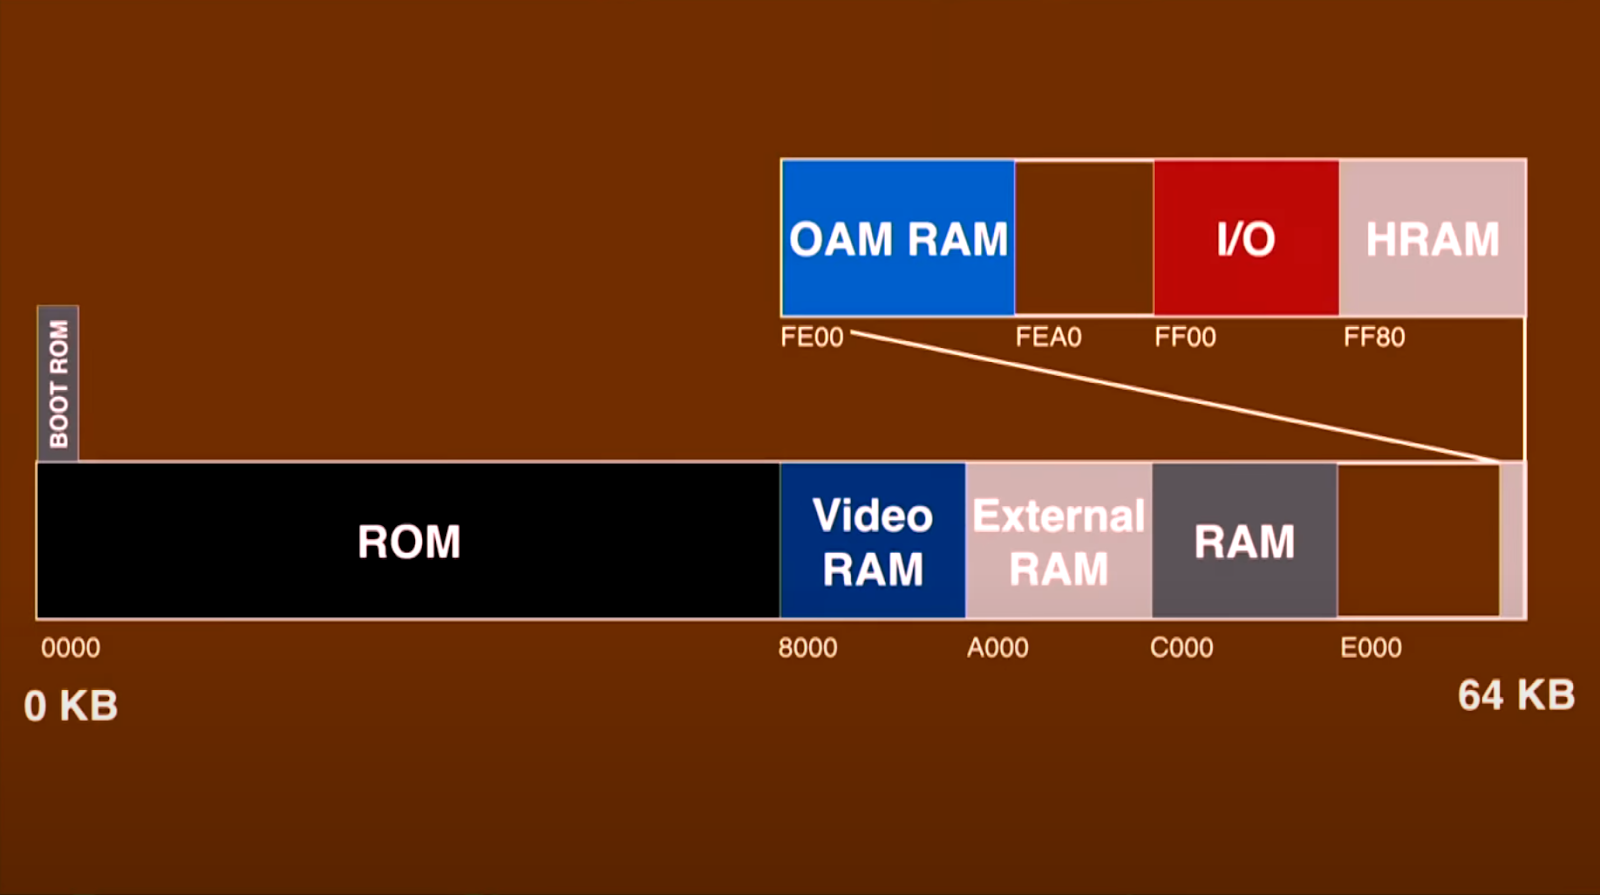
\includegraphics[width=\textwidth]{figures/Memory.png}
    \caption{Displaying the division of different memories in the 64kb address space. \cite{GBTMem}}
    \label{fig:Memory-fig}
\end{figure}  

    
\subsection{The Picture Processing Unit} 
The Picture Processing Unit (PPU) is the module which controls what is displayed on the 160x144 pixel LCD.\cite{pandocsVideo} The video display will be emulated through the use of OpenGL\cite{OpenGL}, which is a free graphical library, and the PPU will tell the display what to render. The PPU is one of the units which due to specifications of the hardware, has some special effects only reproducible if the hardware itself is emulated in certain ways. This module is therefore the most complex module to emulate. %One of these special effects is called 'the wobble-effect' and is made very cool B). possible through the specifics of the PPU. %Making these kinds of emulations possible is a problem in and of itself, and is therefore secondary to making more general progress in emulating more general functionalities.


\subsection{Joypad Input}
To be able to emulate a Game Boy truthfully, one must be able to play the games developed for the console. To do this some kind of controls must be implemented. As this emulator is meant to be designed for PC, the joypad input of the original Game Boy must be emulated. Originally the input is handled through interrupts in the hardware\cite{pandocsinterrupts}\cite{pandocsjoypad}, something which needs to be emulated through the development library SDL\cite{SDL} in order to read the input from a users keyboard.

% use of a graphic library, for example OpenGL, and its functionality for providing input handling.

\subsection{Other hardware modules}

There are of course multiple other hardware modules which can and needs to be emulated to fully reproduce the Game Boy as a system, such as the sound controller. These will currently not be further explored as the main focus is initially to get the main functionality working, which is reading ROMs, rendering, input and gameplay. 
%it does not fit within the scope of this report nor has the development progressed far enough to sufficiently understand the intricacies of them.

% -------Moved to Limitations ------
% \section{The Minimum Viable Product} \todo{I think MVP should only be in limitations /David}
% The Minimum Viable Product (MVP) is the minimum goal set up for providing a solution to the problem. The chosen MVP consists of having a bootable Game Boy emulator which can fully play the simple games, such as Tetris, but without sounds. This will be further explained in section \ref{Limitations}.
%Köra tetris,utan ljud.
% -----------------------------------------
